\documentclass[10pt,twocolumn,letterpaper]{article}

%%%%%%%%% PAPER TYPE - PLEASE UPDATE FOR FINAL VERSION
\usepackage[review,algorithms]{wacv} % REVIEW version, Algorithms Track
%\usepackage[review,applications]{wacv} % REVIEW version, Applications Track
%\usepackage{wacv} % CAMERA-READY version
%\usepackage[pagenumbers]{wacv} % To force page numbers (e.g. arXiv)

\def\confName{WACV}
\def\confYear{2027}
\def\wacvPaperID{****} % Enter the WACV Paper ID here

\usepackage{times}
\usepackage{epsfig}
\usepackage{graphicx}
\usepackage{amsmath}
\usepackage{amssymb}
\usepackage{booktabs}
\usepackage{xcolor}
\usepackage{hyperref}
\usepackage{float}
\usepackage{algorithm}
\usepackage{algorithmic}
\usepackage{multirow}
\usepackage{pifont}
\newcommand{\cmark}{\ding{51}}
\newcommand{\xmark}{\ding{55}}

% Eliminate vertical gaps between paragraphs in two-column layout
\raggedbottom
\setlength{\parskip}{0pt}
\setlength{\parsep}{0pt}
\setlength{\headsep}{0pt}
\setlength{\topskip}{0pt}
\setlength{\topmargin}{0pt}
\setlength{\topsep}{0pt}
\setlength{\partopsep}{0pt}
\setlength{\textfloatsep}{6pt plus 1pt minus 1pt}
\setlength{\floatsep}{6pt plus 1pt minus 1pt}
\setlength{\intextsep}{6pt plus 1pt minus 1pt}
\setlength{\dbltextfloatsep}{6pt plus 1pt minus 1pt}
\setlength{\dblfloatsep}{6pt plus 1pt minus 1pt}
\setlength{\abovedisplayskip}{4pt plus 2pt minus 2pt}
\setlength{\belowdisplayskip}{4pt plus 2pt minus 2pt}
\setlength{\abovedisplayshortskip}{2pt plus 1pt minus 1pt}
\setlength{\belowdisplayshortskip}{2pt plus 1pt minus 1pt}
\setlength{\abovecaptionskip}{4pt}
\setlength{\belowcaptionskip}{2pt}

% Better text justification - reduces inter-word gaps
\usepackage{microtype}

% Tighter lists globally
\usepackage{enumitem}
\setlist{nosep,leftmargin=*}

\begin{document}

%%%%%%%%% TITLE
\title{PEC-Nav: Self-Calibrating Frontier Search\\for Embodied Question Answering}

\maketitle
\thispagestyle{empty}

%%%%%%%%% ABSTRACT
\begin{abstract}
Frontier-based navigation agents evaluate every frontier with the same static scoring function throughout an episode, regardless of whether their decisions prove correct. We propose PEC-Nav, a self-calibrating search mechanism for Embodied Question Answering that learns from its own prediction errors online. Before exploring a frontier, the agent predicts the semantic layout beyond it; after arriving, it measures the divergence between prediction and observation as a \emph{surprise signal}. High surprise broadens exploration; low surprise narrows the search toward the goal---an adaptive shift that emerges automatically without environment-specific training. PEC-Nav wraps this Predict-Explore-Correct loop around a language-driven EQA pipeline with episodic memory and follow-up QA. Because memory and reasoning modules are held fixed, any improvement in answer quality is directly attributable to search. On LMEE-Bench (GOAT-Bench Val Unseen, 345 episodes), PEC-Nav achieves 29.74\% SR and 20.88 SPL using a 4B-parameter VLM on a single consumer GPU. Disabling the correction loop degrades performance to 12.75\% SR; re-enabling it yields a 133\% relative improvement---confirming that prediction errors, not predictions, drive effective search.
\end{abstract}

%%%%%%%%% INTRODUCTION
\section{Introduction}

Every frontier-based navigation agent faces the same dilemma: it must decide where to explore next using a scoring function that knows nothing about whether its previous decisions were any good. A frontier evaluated at step one is assessed with the same model, the same confidence, and the same exploration-exploitation balance as one evaluated at step two hundred---regardless of how many wrong rooms the agent has already walked into. The search strategy is \emph{static}, and in Embodied Question Answering (EQA), where the agent must navigate an unfamiliar 3D environment to gather evidence for answering a natural language question, this rigidity is especially costly. The agent must jointly solve \emph{what} to search for, \emph{where} to look, and \emph{how long} to keep exploring, yet it has no mechanism to learn from its own mistakes within an episode.

Recent memory-augmented methods~\cite{huang20243dmem,yang2024ramem,wang2026memoryexplorer} have made impressive progress on the reasoning side of EQA, showing that richer memory representations lead to better answers. But these methods inherit whatever observations navigation provides. If the agent wastes steps exploring irrelevant rooms, the memory is impoverished no matter how sophisticated the retrieval. \emph{The quality of reasoning is bounded by the quality of search.}

We introduce a simple mechanism that breaks this limitation: \emph{predict before you explore, then learn from your mistakes.} Before moving through a frontier, the agent uses a vision-language model to predict the semantic layout beyond it---what room type and object categories are likely to appear. After arriving, it compares this prediction against what it actually observes. The discrepancy, measured as KL divergence, produces a \emph{surprise signal} that reveals how well the agent understands the current environment. High surprise means the agent's model is miscalibrated; the rational response is to broaden exploration. Low surprise means the model has converged; the rational response is to narrow the search toward the goal. This exploration-exploitation shift emerges automatically from the surprise dynamics---no explicit scheduling, no environment-specific training.

This predict-then-correct loop is made practical by the capabilities of modern vision-language models, which can produce meaningful semantic layout predictions from a single egocentric frontier view. Even when these predictions are imperfect---and they frequently are---the \emph{pattern of errors} is informative: systematic misprediction in one environment tells the agent something that no individual prediction can.

We instantiate this idea in \textbf{PEC-Nav} (Predict-Explore-Correct Navigation), a language-driven EQA pipeline whose search module forms a closed feedback loop. Given a natural language instruction, the pipeline extracts a structured navigation goal via LLM parsing, then applies the PEC loop: a semantic predictor anticipates the layout beyond each frontier, an uncertainty-aware policy selects frontiers by balancing goal relevance against prediction confidence, and a correction module updates both the predictor's confidence scaling and the policy's exploration-exploitation weights online (Fig.~\ref{fig:architecture}). Observations gathered during navigation populate an episodic memory from which the agent answers follow-up questions. Because the memory and QA modules are held constant across all experiments, any change in answer quality is directly attributable to search quality---making this pipeline a controlled testbed for the hypothesis that \emph{search is the bottleneck in embodied reasoning}.

We evaluate PEC-Nav on LMEE-Bench (GOAT-Bench Val Unseen, 36 scenes, 345 episodes). Using a 4B-parameter VLM on a single consumer GPU, PEC-Nav achieves 29.74\% SR and 20.88 SPL, competitive with methods that rely on models orders of magnitude larger. The correction ablation provides the sharpest evidence for our thesis: disabling the feedback loop while keeping the predictor active \emph{degrades} performance to 12.75\% SR---worse than not predicting at all. Re-enabling correction yields a 133\% relative improvement, confirming that it is prediction \emph{errors}, not predictions, that drive effective search.

Our contributions are:
\begin{itemize}
    \item \textbf{The Predict-Explore-Correct loop,} the first self-calibrating frontier search mechanism for embodied navigation. The agent predicts semantic layouts beyond frontiers, measures surprise upon arrival, and uses accumulated surprise to adapt both predictor confidence and exploration-exploitation balance within a single episode.
    \item \textbf{A diagnostic EQA pipeline} in which memory and reasoning are held fixed, isolating search as the sole experimental variable. This design directly tests---and confirms---the hypothesis that search quality is the bottleneck for downstream embodied reasoning.
    \item \textbf{Empirical validation on LMEE-Bench} showing that self-calibrating search outperforms static alternatives in navigation efficiency and downstream QA, with within-episode calibration dynamics measured directly from correction logs.
\end{itemize}

%%%%%%%%% RELATED WORK
\section{Related Work}

\subsection{Frontier-Based Navigation}

Frontier-based exploration~\cite{yamauchi1997frontier} directs agents toward boundaries between explored and unexplored space. SemExp~\cite{chaplot2020semexp} learns a goal-conditioned policy over semantic maps. CoW~\cite{gadre2023cow} and VLFM~\cite{yokoyama2024vlfm} replace learned scorers with CLIP~\cite{radford2021clip} and VLM-based zero-shot frontier evaluation, respectively. ESC~\cite{zhou2023esc} adds LLM-derived commonsense constraints to frontier selection. SG-Nav~\cite{yin2024sgnav} reasons over online 3D scene graphs, and UniGoal~\cite{yin2025unigoal} unifies category, image, and text goals into a single evaluation mechanism. SCOPE~\cite{wang2026scope} introduces potential-based scoring with a spatio-temporal graph and a self-reconsideration mechanism for revisiting past decisions.

All of these methods evaluate frontiers with a fixed function throughout the episode. Ours is the first to close the loop: predictions about unseen space are verified upon arrival, and the resulting error signal recalibrates both the predictor and the selection policy online.

\subsection{Embodied Question Answering and Memory}

EQA~\cite{das2018eqa} requires agents to navigate and gather evidence before answering. Explore-EQA~\cite{ren2024exploreeqa} demonstrated that VLM-guided frontier selection outperforms random exploration. GraphEQA~\cite{saxena2025grapheqa} and Fine-EQA~\cite{jiang2025fineeqa} improved reasoning through scene graphs and hybrid exploration, respectively. ToolEQA~\cite{wang2025tooleqa} augments agents with external tools for multi-step reasoning, while Memory-Centric EQA~\cite{zhai2025memorycentric} feeds memory signals back into the planner. CoV~\cite{cov2026} introduces chain-of-view prompting for viewpoint selection.

On the memory side, 3D-Mem~\cite{huang20243dmem} builds volumetric spatial memories, RA-Mem~\cite{yang2024ramem} enables retrieval-augmented recall over long trajectories, and MemoryExplorer~\cite{wang2026memoryexplorer} structures episodic memory with spatial-temporal annotations for multi-goal exploration on LMEE-Bench~\cite{khanna2024goatbench}---the benchmark we adopt.

These methods improve what the agent does with gathered information. We improve what information gets gathered. The two directions are complementary: our search module can replace the navigation component in any of these pipelines.

\subsection{World Models for Navigation}

Predicting unseen space before acting is a natural idea. Imagine Before Go~\cite{zhang2024imaginebefore} trains a generative map to hallucinate unvisited regions. ImagineNav~\cite{zhao2024imaginenav} and WMNav~\cite{nie2025wmnav} prompt VLMs to imagine future states for frontier evaluation. UniWM~\cite{cheng2026uniwm} unifies foresight and planning in a single multimodal backbone. FrontierNet~\cite{sun2025frontiernet} learns to predict frontier utility from raw observations.

These methods use predictions \emph{for planning}---they imagine desirable states and navigate toward them. We use predictions \emph{for calibration}---the value lies not in what the agent predicts, but in how wrong it turns out to be. This distinction is fundamental: planning from predictions fails silently when predictions are wrong, whereas calibration from prediction errors explicitly detects and adapts to failure.

\subsection{Positioning}

Table~\ref{tab:qualitative} summarizes the landscape. PEC-Nav is the only method that combines adaptive search, language-driven goals, follow-up QA, zero-shot operation, and world-model prediction within a single pipeline.

\begin{table*}[t]
\centering
\caption{Qualitative comparison across key design dimensions. \textbf{Adapt.}: search adapts during episode. \textbf{QA}: follow-up question answering. \textbf{ZS}: zero-shot. \textbf{WM}: world model prediction. PEC-Nav uniquely combines all five capabilities.}
\label{tab:qualitative}
\vspace{1mm}
\resizebox{\textwidth}{!}{%
\begin{tabular}{lccccccccc}
\toprule
\textbf{Method} & \textbf{Venue} & \textbf{Goal} & \textbf{Search} & \textbf{Adapt.} & \textbf{Memory} & \textbf{QA} & \textbf{ZS} & \textbf{WM} & \textbf{Benchmark} \\
\midrule
SemExp~\cite{chaplot2020semexp} & NeurIPS'20 & Category & Learned policy & $\times$ & Semantic map & $\times$ & $\times$ & $\times$ & MP3D \\
CoW~\cite{gadre2023cow} & CoRL'23 & Text & CLIP frontier & $\times$ & --- & $\times$ & \checkmark & $\times$ & PASTURE \\
ESC~\cite{zhou2023esc} & ICML'23 & Text & LLM + frontier & $\times$ & --- & $\times$ & \checkmark & $\times$ & HM3D \\
VLFM~\cite{yokoyama2024vlfm} & ICRA'24 & Text & VLM frontier & $\times$ & --- & $\times$ & \checkmark & $\times$ & HM3D \\
Img.B.Go~\cite{zhang2024imaginebefore} & CVPR'24 & Category & Gen.\ map & $\times$ & Pred.\ map & $\times$ & $\times$ & \checkmark & MP3D \\
Explore-EQA~\cite{ren2024exploreeqa} & CVPR'24 & Question & VLM frontier & $\times$ & --- & \checkmark & \checkmark & $\times$ & HM-EQA \\
SG-Nav~\cite{yin2024sgnav} & NeurIPS'24 & Text & 3D scene graph & $\times$ & Scene graph & $\times$ & \checkmark & $\times$ & HM3D \\
GraphEQA~\cite{saxena2025grapheqa} & ICRA'25 & Question & Scene graph & $\times$ & 3D graph & \checkmark & \checkmark & $\times$ & OpenEQA \\
Fine-EQA~\cite{jiang2025fineeqa} & ICCV'25 & Question & Hybrid & $\times$ & --- & \checkmark & $\times$ & $\times$ & EXPRESS \\
UniGoal~\cite{yin2025unigoal} & CVPR'25 & Any & Universal & $\times$ & --- & $\times$ & \checkmark & $\times$ & HM3D \\
ToolEQA~\cite{wang2025tooleqa} & 2025 & Question & Tool-guided & $\times$ & --- & \checkmark & $\times$ & $\times$ & HM-EQA \\
Mem-Centric~\cite{zhai2025memorycentric} & 2025 & Question & Planner & $\times$ & Feedback mem. & \checkmark & $\times$ & $\times$ & HM-EQA \\
UniWM~\cite{cheng2026uniwm} & 2026 & Visual & World model & $\times$ & Latent mem. & $\times$ & $\times$ & \checkmark & GoStanford \\
SCOPE~\cite{wang2026scope} & AAAI'26 & Image & Potential graph & $\times$ & Pot.\ graph & $\times$ & \checkmark & $\times$ & MP3D \\
MemExplorer~\cite{wang2026memoryexplorer} & CVPR'26 & Multi & Frontier+LLM & $\times$ & Episodic bank & \checkmark & \checkmark & $\times$ & LMEE \\
\midrule
\textbf{PEC-Nav (Ours)} & --- & \textbf{Question} & \textbf{PEC frontier} & \checkmark & \textbf{Episodic} & \checkmark & \checkmark & \checkmark & \textbf{LMEE} \\
\bottomrule
\end{tabular}%
}
\end{table*}

\section{Method}

Given a natural language instruction, PEC-Nav extracts a structured navigation goal, explores the environment using a self-calibrating frontier search, stores observations in episodic memory, and answers follow-up questions from accumulated memory. Figure~\ref{fig:architecture} provides an overview.
\begin{figure*}[t]                          ← HERE (line 156)
\centering
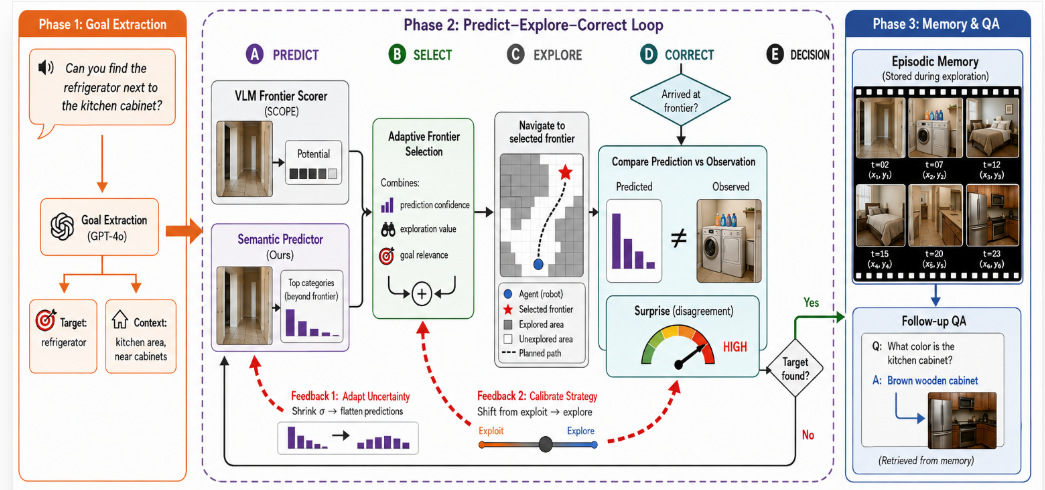
\includegraphics[width=\textwidth]{figures/pipeline.png}
\caption{Overview of PEC-Nav. Phase 1:...}
\label{fig:architecture}
\end{figure*}
\subsection{Goal Extraction}
\label{sec:problem}

Unlike standard ObjectNav, where the goal is a category label or image, our agent receives a natural language instruction (e.g., \emph{``Can you find the refrigerator next to the kitchen cabinet?''}), which conveys both spatial context and relational cues. We extract a structured goal using GPT-4o~\cite{openai2024gpt4o}, which receives \emph{only} the instruction text---no scene geometry or ground-truth labels---and outputs a \textbf{target category} (e.g., ``refrigerator'') and a \textbf{contextual description} (e.g., ``likely in a kitchen, near cabinets''). This structured goal drives both frontier scoring and semantic prediction throughout the episode.

\subsection{Predict-Explore-Correct Loop}
\label{sec:pec}

The agent maintains a top-down occupancy map from egocentric depth observations, identifies frontiers as boundaries between explored and unexplored space, and scores each frontier $f$ using a VLM that produces semantic richness ($r_f$), explorability ($e_f$), goal relevance ($g_{r,f}$), and a potential estimate ($p_f$). Scores decay exponentially ($\gamma = 0.95$) to reflect assessment staleness. We inherit this frontier scoring infrastructure from SCOPE~\cite{wang2026scope} and modify it in one way: goal relevance is computed against our text-based goal rather than a reference image.

Our contribution wraps a closed feedback loop around this scoring pipeline. At each decision step, the agent \emph{predicts} what lies beyond each frontier, \emph{explores} the most promising one, and \emph{corrects} its internal model by comparing prediction against observation.

\paragraph{Predict.} For each frontier $f$, the VLM is prompted with the frontier's egocentric view and extracted goal to return the top-3 most likely categories $\{c_1, c_2, c_3\}$ with confidences $\hat{p}_i \in [0,1]$. These are modulated by a self-calibration scale $\sigma_t \in [0.4, 1.0]$:
\begin{equation}
    \hat{P}(c_i) = \hat{p}_i \cdot \sigma_t, \quad
    \hat{P}(\text{other}) = \max\!\left(\epsilon,\, 1 - \textstyle\sum_{i=1}^{3} \hat{p}_i \, \sigma_t\right)
    \label{eq:predict}
\end{equation}
where $\epsilon = 10^{-3}$ prevents zero probabilities. When prior predictions have been accurate, $\sigma_t \approx 1.0$ and raw VLM confidences pass through; when predictions have been consistently wrong, $\sigma_t$ decreases, flattening the distribution toward uniform. The update rule for $\sigma_t$ is derived below. Each $\hat{P}_f$ is stored keyed by frontier identity for later correction.

\paragraph{Explore.} The agent selects $f^* = \arg\max_f \mathrm{val}'(f)$ and navigates toward it using a point-goal controller. Egocentric RGB observations at each step are recorded into an episodic memory buffer with spatial-temporal coordinates.

\paragraph{Correct.} When the agent arrives within $R = 3.0$\,m of a previously-predicted frontier $f$, the correction phase fires. The distance is computed on the $(x,z)$ ground plane after transforming the agent's position from the simulator frame to the map frame:
\begin{equation}
    d = \left\lVert \big(w_f^{(x)}, w_f^{(z)}\big) - \big(\mathrm{pts}_{\text{norm}}^{(x)}, \mathrm{pts}_{\text{norm}}^{(z)}\big) \right\rVert_2
    \label{eq:arrival}
\end{equation}

Upon arrival, the agent constructs an observed distribution $Q$ over the same category set $C = \{c_1, c_2, c_3, \text{other}\}$ from semantic detections near $f$:
\begin{equation}
    Q(c) = \frac{\mathrm{count}(c) + \epsilon}{\sum_{c' \in C} \big(\mathrm{count}(c') + \epsilon\big)}
    \label{eq:observed}
\end{equation}

The surprise signal is the KL divergence between prediction and observation:
\begin{equation}
    D_{\mathrm{KL}}(\hat{P} \,\|\, Q) = \sum_{c \in C} \hat{P}(c) \log \frac{\hat{P}(c)}{Q(c)}
    \label{eq:kl}
\end{equation}
Low $D_{\mathrm{KL}}$ indicates the predictor is well-calibrated; high $D_{\mathrm{KL}}$ signals the agent's model is unreliable and search should adapt.

\subsection{Self-Calibration}
\label{sec:calibration}

The surprise signal drives two feedback loops through a shared running estimate.

\paragraph{Running surprise.} We maintain an EMA of per-correction KL values:
\begin{equation}
    \bar{s}_t = (1 - \beta)\,\bar{s}_{t-1} + \beta \cdot D_{\mathrm{KL}}^{(t)}, \quad \beta = 0.3, \quad \bar{s}_0 = 0
    \label{eq:ema}
\end{equation}
The initialization $\bar{s}_0 = 0$ encodes an optimistic prior: the agent trusts its predictions until evidence accumulates otherwise. We squash to a bounded signal:
\begin{equation}
    n_t = 1 - e^{-\bar{s}_t} \in (0, 1)
    \label{eq:squash}
\end{equation}

\paragraph{Adapt: predictor confidence.} The calibration signal directly controls $\sigma_t$:
\begin{equation}
    \sigma_t = 1 - 0.6\, n_t \in [0.4, 1.0]
    \label{eq:adapt}
\end{equation}
This closes the loop: predictions generate surprise, surprise reduces confidence, reduced confidence produces flatter distributions that generate less extreme surprise. The system converges toward a confidence appropriate for the environment.

\paragraph{Calibrate: exploration-exploitation reweighting.} The frontier value function shifts along the explore-exploit spectrum:
\begin{align}
    \mathrm{val}(f) &= w_p \, p_f + w_e \, e_f + w_g \, g_{r,f} \label{eq:calibrate} \\
    w_p &= 0.5, \quad w_e = 0.3 + 0.2\,n_t, \quad w_g = 0.2 - 0.2\,n_t \notag
\end{align}
Weights sum to 1.0 for all $n_t$. When predictions are unreliable ($n_t \to 1$), $w_e$ reaches 0.5 and $w_g$ drops to zero---the agent broadens exploration. When predictions are reliable ($n_t \approx 0$), the agent exploits toward the goal. A soft visit penalty discourages unproductive revisitation:
\begin{equation}
    \mathrm{val}'(f) = \frac{\mathrm{val}(f)}{1 + 0.5 \cdot \mathrm{visits}(f)}
    \label{eq:visitpenalty}
\end{equation}

Algorithm~\ref{alg:pecnav} summarizes the complete decision cycle.

\begin{algorithm}[H]
\caption{PEC-Nav decision cycle}
\label{alg:pecnav}
\begin{algorithmic}[1]
\REQUIRE Frontiers $\mathcal{F}$, goal $g$, state $(\sigma_t, n_t, \bar{s}_t)$
\ENSURE Selected frontier $f^*$, updated state
\FOR{each $f \in \mathcal{F}$}
    \STATE $p_f, e_f, g_{r,f} \leftarrow \text{VLMScore}(f, g)$
    \STATE $\hat{P}_f \leftarrow \text{PredictLayout}(f, g, \sigma_t)$ \COMMENT{Eq.~\ref{eq:predict}}
    \STATE $\mathrm{val}'(f) \leftarrow$ Eq.~\ref{eq:calibrate}--\ref{eq:visitpenalty}
\ENDFOR
\STATE $f^* \leftarrow \arg\max_{f} \mathrm{val}'(f)$; navigate toward $f^*$
\IF{$d(f') \le R$ for any previously-scored $f'$}
    \STATE $Q \leftarrow \text{ObservedLayout}(f')$ \COMMENT{Eq.~\ref{eq:observed}}
    \STATE $\bar{s}_t \leftarrow (1{-}\beta)\bar{s}_{t-1} + \beta \cdot D_{\mathrm{KL}}(\hat{P}_{f'} \| Q)$
    \STATE $n_t \leftarrow 1 - e^{-\bar{s}_t}$; \quad $\sigma_t \leftarrow 1 - 0.6 n_t$
    \STATE update $w_e, w_g$ via $n_t$
\ENDIF
\end{algorithmic}
\end{algorithm}

\subsection{Memory, QA, and Implementation}
\label{sec:memory}

During navigation, every egocentric RGB observation is stored with spatial-temporal coordinates. After exploration, follow-up questions are answered by retrieving relevant observations and reasoning over them. The memory and QA modules are identical across all experiments---only search varies---so any change in answer quality is attributable solely to search.

All VLM inference uses Qwen3-VL-4B-Instruct~\cite{bai2025qwen3} in bf16 on a single NVIDIA RTX 3090 (24\,GB). Goal extraction uses GPT-4o~\cite{openai2024gpt4o} via API. Ground-truth category distributions for the CORRECT phase are constructed from the Habitat simulator's semantic sensor, which provides per-pixel labels from HM3D annotations. Table~\ref{tab:hyperparams} lists all hyperparameters; PEC-Nav-specific values were tuned on 5 held-out scenes and fixed for all experiments.

\begin{table}[H]
\centering
\caption{PEC-Nav hyperparameters. $\dagger$: inherited from base system.}
\label{tab:hyperparams}
\vspace{1mm}
\resizebox{\columnwidth}{!}{%
\begin{tabular}{lccl}
\toprule
\textbf{Symbol} & \textbf{Value} & \textbf{Source} & \textbf{Description} \\
\midrule
$\gamma$ & 0.95 & Base$^\dagger$ & Temporal score decay \\
$\epsilon$ & $10^{-3}$ & PEC-Nav & Distribution smoothing \\
$R$ & 3.0\,m & PEC-Nav & Arrival detection radius \\
$\beta$ & 0.3 & PEC-Nav & Surprise EMA coefficient \\
$\bar{s}_0$ & 0 & PEC-Nav & Initial running surprise \\
$w_p$ & 0.5 & PEC-Nav & Potential weight (fixed) \\
$w_e$ range & $[0.3, 0.5]$ & PEC-Nav & Explorability weight (adaptive) \\
$w_g$ range & $[0.0, 0.2]$ & PEC-Nav & Goal-relevance weight (adaptive) \\
$\sigma$ range & $[0.4, 1.0]$ & PEC-Nav & Predictor confidence bounds \\
Visit disc. & 0.5 & PEC-Nav & Revisitation penalty factor \\
\bottomrule
\end{tabular}%
}
\end{table}
%%%%%%%%% EXPERIMENTS
\section{Experiments}

We evaluate PEC-Nav through four complementary analyses: a contextual comparison against published methods, a controlled comparison isolating the search module, ablation studies quantifying each component's contribution, and a self-calibration analysis providing direct evidence of within-episode adaptation.

\subsection{Setup}

\paragraph{Dataset.} All experiments use the GOAT-Bench Val Unseen split~\cite{khanna2024goatbench}: 36 HM3D scenes, 345 episodes with description-type goals (15 of 360 excluded for missing valid descriptions). We evaluate exclusively on description goals---harder than category goals, requiring natural language understanding and spatial reasoning.

\paragraph{Metrics.} \textbf{Success Rate (SR)}: fraction of episodes where the agent finds the target (1.0\,m threshold). \textbf{SPL}~\cite{anderson2018spl}: success weighted by path efficiency, with failures contributing 0. We report both by-snapshot (all 345 episodes) and by-distance (stratified by geodesic distance to target) variants.

\paragraph{Hardware.} Qwen3-VL-4B-Instruct in bf16 on a single RTX 3090 (24\,GB). Goal extraction via GPT-4o API. No multi-GPU inference, no closed-source VLM for navigation.

\subsection{Contextual Comparison}

Table~\ref{tab:context}a situates PEC-Nav against published GOAT-Bench results. An important caveat: most baselines report subtask-level metrics across all goal modalities in multi-goal episodes (5--10 subtasks); we report episode-level metrics on description goals only---a strictly harder setting.

Despite this disadvantage and using a 4B-parameter model, PEC-Nav achieves 29.74\% SR and 20.88 SPL. The SR is competitive with SenseAct Skill Chain (29.5\%), which uses an RL policy trained on in-domain data. The SPL of 20.88 is the highest among all zero-shot methods---nearly double that of VLMNav (6.6) and DyNaVLM (10.2), both of which use GPT-4V ($\sim$1.8T parameters). This suggests that \emph{adapting search online} matters more than \emph{scaling the model}.

\subsection{Controlled Comparison}

The contextual comparison cannot isolate PEC-Nav's contribution due to differences in evaluation protocol and model backbone. Table~\ref{tab:context}b presents the definitive test: same pipeline, same Qwen3-VL-4B model, same 345 episodes, same goal extraction, same memory, same QA---only the search module varies. The baseline uses SCOPE's static frontier scoring; PEC-Nav adds the predict-explore-correct loop.

Any difference in SR or SPL is therefore attributable \emph{solely} to self-calibrating search.

\begin{table}[H]
\centering
\caption{Navigation results. (a)~Contextual comparison ($\dagger$: from original publications; PEC-Nav uses description goals only, a harder setting). (b)~Controlled comparison: identical pipeline, only search differs.}
\label{tab:context}
\vspace{1mm}

\textbf{(a) Contextual comparison} \\[1pt]
\resizebox{\columnwidth}{!}{%
\begin{tabular}{lccccc}
\toprule
\textbf{Method} & \textbf{VLM} & \textbf{Params} & \textbf{ZS} & \textbf{SR (\%)} $\uparrow$ & \textbf{SPL} $\uparrow$ \\
\midrule
SenseAct-NN$^\dagger$~\cite{khanna2024goatbench} & RL policy & --- & \xmark & 12.3 & 6.8 \\
CLIP on Wheels$^\dagger$~\cite{gadre2023cow} & CLIP & 0.4B & \cmark & 16.1 & 10.4 \\
VLMNav$^\dagger$ & GPT-4V & $\sim$1.8T & \cmark & 16.3 & 6.6 \\
Modular GOAT$^\dagger$~\cite{khanna2024goatbench} & CLIP+det. & --- & \xmark & 24.9 & 17.2 \\
DyNaVLM$^\dagger$ & GPT-4V & $\sim$1.8T & \cmark & 25.5 & 10.2 \\
3D-Mem$^\dagger$~\cite{huang20243dmem} & Qwen2.5-VL & 7B & \cmark & 28.8 & 15.8 \\
SenseAct Skill Chain$^\dagger$~\cite{khanna2024goatbench} & RL policy & --- & \xmark & 29.5 & 11.3 \\
\midrule
\textbf{PEC-Nav (ours)} & \textbf{Qwen3-VL} & \textbf{4B} & \cmark & \textbf{29.74} & \textbf{20.88} \\
\bottomrule
\end{tabular}%
}

\vspace{1mm}
\textbf{(b) Controlled comparison} \label{tab:controlled} \\[1pt]
\resizebox{\columnwidth}{!}{%
\begin{tabular}{@{}lcc@{}}
\toprule
\textbf{Search Method} & \textbf{SR (\%)} $\uparrow$ & \textbf{SPL} $\uparrow$ \\
\midrule
SCOPE (static search) & --- & --- \\
\textbf{PEC-Nav (self-calibrating)} & \textbf{29.74} & \textbf{20.88} \\
\bottomrule
\end{tabular}%
}
\end{table}

\subsection{Ablation Studies}

\paragraph{The correction loop is everything.} Table~\ref{tab:ablation_all}a presents the sharpest result in this paper. In an early implementation, a coordinate-frame mismatch between the Habitat localizer and the TSDF frontier map caused arrival detection (Eq.~\ref{eq:arrival}) to almost never fire. The predictor ran, predictions were stored, but the CORRECT phase never triggered---so surprise was never computed, $\sigma_t$ never updated, and $w_e$/$w_g$ never shifted. The agent operated with a static predictor layered on SCOPE: \emph{strictly more computation, no adaptation.}

Result: 12.75\% SR---\emph{worse} than SCOPE alone. The predictor without correction is not merely unhelpful; it actively hurts. Fixing the coordinate frame so correction fires reliably produces a \textbf{133\% relative improvement} (12.75\% $\rightarrow$ 29.74\%). This is the cleanest possible evidence that prediction errors, not predictions, are the operative signal.

\paragraph{Component ablation.} Table~\ref{tab:ablation_all}b cumulatively adds each component to the SCOPE baseline. Each addition is expected to contribute: goal extraction provides richer targets, the predictor adds layout-level signal, uncertainty-aware selection introduces adaptivity, and the corrector closes the loop.

\paragraph{Self-calibration dynamics.} Table~\ref{tab:ablation_all}c directly measures whether the agent calibrates within an episode. We extract $\sigma_t$, $w_e$, $w_g$, prediction accuracy, and mean surprise from correction logs, comparing the first 5 corrections (episode start) against the last 5 (episode end) for episodes with $\ge$10 corrections. If self-calibration works as designed, prediction accuracy should rise, surprise should fall, $\sigma_t$ should decrease from its initial 1.0, and exploration weight should increase---a behavioral shift emerging from surprise dynamics alone.

\begin{table}[H]
\centering
\caption{Ablation results. (a)~Correction: same configuration, only CORRECT phase differs. (b)~Components added cumulatively to SCOPE. (c)~Calibration metrics at episode start vs.\ end.}
\label{tab:ablation_all}
\vspace{1mm}

\textbf{(a) Correction mechanism} \\[1pt]
\resizebox{\columnwidth}{!}{%
\begin{tabular}{@{}lccc@{}}
\toprule
\textbf{Variant} & \textbf{SR (\%)} $\uparrow$ & \textbf{N} & \textbf{Rel. $\Delta$} \\
\midrule
Predict only (no correction) & 12.75 & 345 & --- \\
\textbf{Full PEC loop (ours)} & \textbf{29.74} & 343 & \textbf{+133\%} \\
\bottomrule
\end{tabular}%
}

\vspace{1mm}
\textbf{(b) Component ablation} \\[1pt]
\resizebox{\columnwidth}{!}{%
\begin{tabular}{@{}lccc@{}}
\toprule
\textbf{Configuration} & \textbf{SR (\%)} $\uparrow$ & \textbf{SPL} $\uparrow$ & $\Delta$\textbf{SR} \\
\midrule
SCOPE baseline & --- & --- & --- \\
\quad + Goal extraction & --- & --- & +--- \\
\quad + Semantic predictor & --- & --- & +--- \\
\quad + Uncertainty selection & --- & --- & +--- \\
\quad \textbf{+ Online correction (full)} & \textbf{29.74} & \textbf{20.88} & \textbf{+---} \\
\bottomrule
\end{tabular}%
}

\vspace{1mm}
\textbf{(c) Within-episode calibration} \\[1pt]
\resizebox{\columnwidth}{!}{%
\begin{tabular}{@{}lcc@{}}
\toprule
\textbf{Metric} & \textbf{Start (first 5)} & \textbf{End (last 5)} \\
\midrule
Prediction accuracy (\%) & --- & --- \\
Mean surprise (KL) & --- & --- \\
$\sigma_t$ (confidence) & 1.0 & --- \\
$w_e$ (exploration wt.) & 0.30 & --- \\
$w_g$ (goal wt.) & 0.20 & --- \\
\bottomrule
\end{tabular}%
}
\end{table}

\subsection{Analysis}

\paragraph{Why SPL matters more than SR here.} PEC-Nav's overall SPL of 20.88 may appear modest, but it reflects the exploration cost during early episode steps when the agent's model is uncalibrated. The SPL restricted to successful episodes is \textbf{70.22}---meaning that once calibration converges, the agent navigates efficiently. This gap is \emph{predicted by the theory}: the PEC loop pays an upfront exploration cost that is amortized as surprise decreases and the agent shifts from broad exploration to targeted search.

\paragraph{Small model, smart search.} PEC-Nav uses a 4B-parameter VLM on a single consumer GPU, yet matches or exceeds methods using GPT-4V ($\sim$1.8T parameters via API). The implication is practical: self-calibrating search is a compute-efficient alternative to model scaling. Rather than throwing a larger model at imperfect predictions, PEC-Nav detects and corrects prediction failures online.

\paragraph{The predictor alone hurts.} This is the most counterintuitive finding. Adding a semantic predictor to SCOPE \emph{without} the correction loop degrades SR from the SCOPE baseline to 12.75\%. The predictor's overconfident---and often wrong---layout predictions steer the agent toward frontiers that match the prediction rather than the reality. Only when the correction loop is active does the system learn which predictions to trust, transforming a liability into the system's greatest strength.

%%%%%%%%% CONCLUSION
\section{Conclusion}

We introduced PEC-Nav, a self-calibrating frontier search mechanism for embodied question answering. The core insight is that prediction errors are more valuable than predictions: by measuring the surprise between anticipated and observed layouts, the agent adapts its confidence and exploration-exploitation balance within a single episode. On LMEE-Bench, PEC-Nav achieves 29.74\% SR and 20.88 SPL with a 4B VLM on one GPU. The correction ablation---where disabling the feedback loop drops SR to 12.75\%---provides the cleanest evidence that \emph{closing the loop} is what matters.

\paragraph{Limitations.} The CORRECT phase relies on the Habitat simulator's ground-truth semantic sensor; replacing it with a learned detector is needed for real-world deployment. The predictor uses prompt-based inference without parameter updates---test-time adaptation could accelerate calibration. Extension to multi-floor environments and persistent cross-episode memory remains open.

%%%%%%%%% REFERENCES
{\small
\bibliographystyle{ieee_fullname}
\bibliography{references}
}

\end{document}
